\documentclass[12pt]{article}
\usepackage{mathtools}
\addtolength{\textheight}{.5in}
\addtolength{\textwidth}{1in}
\addtolength{\topmargin}{-.25in}
\addtolength{\evensidemargin}{-.5in}
\addtolength{\oddsidemargin}{-.5in}
\usepackage{listings}
\lstset{
  basicstyle=\small\ttfamily,
  frame=lrtb,
  showstringspaces=false,
}
\begin{document}

\title{PHY 267 HW 5}
\author{Imran Hasan}
\maketitle

\section{Scheter Function}
\subsection{$\phi$(M)dM}
For the Scheter function we have $\phi(L)\mathrm{d}L = n_{*} (\frac{L}{L_*})^{\alpha} \exp(-L/L_{*}) \mathrm{d}\big(\frac{L}{L_*}\big)$ with the relationship $\log(\frac{L}{L_*}) = -0.4(M - M_{*})$. Changing variables we can write

$$(\frac{L}{L_*}) = 10^{-0.4(M - M_{*})} $$

$$\frac{1}{(\frac{L}{L_*}) \ln 10} \mathrm{d}\Big(\frac{L}{L_*}\Big) = -0.4\mathrm{d}M$$

$$ \phi(M)\mathrm{d}M = -0.4 \ln 10 n_{*}10^{-0.4 (\alpha + 1) (M - M_{*})} \exp(10^{-0.4(M - M_{*})})  \mathrm{d}M$$

\subsection{scaling relations}
We have $n(L) \mathrm{d} L = \phi(L) V_{s}(L) \mathrm{d}L$ with $ d \propto L^{1/2}$ and $V_{s} \propto d^3 \propto L^{3/2} $. Swapping in the Scheter function and using the scaling relation for Volume, we can write

$$n(L) \propto n_{*} (\frac{L}{L_*})^{\alpha + 3/2} \exp(-L/L_{*})$$

We can find extrema for this function by taking the derivative and setting it equal to zero. This will give 

$$ n_{*} (\alpha + 3/2) L_{*}^{-1} (\frac{L}{L_*})^{\alpha + 1/2} \exp(-L/L_{*}) -  n_{*} (\frac{L}{L_*})^{\alpha + 3/2} \exp(-L/L_{*}) L_{*}^{-1}= 0$$

$$  (\alpha + 3/2)  (\frac{L}{L_*})^{\alpha + 1/2} =  (\frac{L}{L_*})^{\alpha + 3/2}  $$

$$ \alpha + 3/2   =  \frac{L}{L_*} $$

For our case where $\alpha$ = -1.25 we have 
$$\frac{L}{L_*} = .25$$ 
\subsection{Mass to light ratio}
If we weight the Scheter function by Luminosity we can get a Luminosity density. We can then use the mass to light ratio to turn this into a mass density. To do the integral, let x = $\frac{L}{L_*}$. Then the luminosity density for our setting becomes 

$$ \int^{\infty}_0 L \phi(L) \mathrm{d}L = n_* \int^{\infty}_0 (L/L_*)^{-.25} \exp(-L/L_*) \mathrm{d}(\frac{L}{L_*}) $$
$$ n_* \int^{\infty}_0 x^{-.25} \exp(-2.5 x) \mathrm{d}x  = 1.23 \times n_* $$

This result is in units of $L_{*}$. If we take $L_{*} = 10^{10} h^{-2} L_{\odot}$, $n_{*} =0.012 h$, $h = 0.7$, along with the mass to light ratio, we can convert this into a mass density. 

$$ 50 \times 10^{10} \times .7^{-2} \times1.23 \times 0.012 \times .07 \,M_{\odot}  \mathrm{Mpc}^{-3} = 1.05 \times 10^9 M_{\odot} \mathrm{Mpc}^{-3} $$ or about $6.67 \times 10^{-32} \mathrm{g/cm}^3$

\subsection{Scheter functions}
Please see figure 1 below
\begin{figure}
\centering
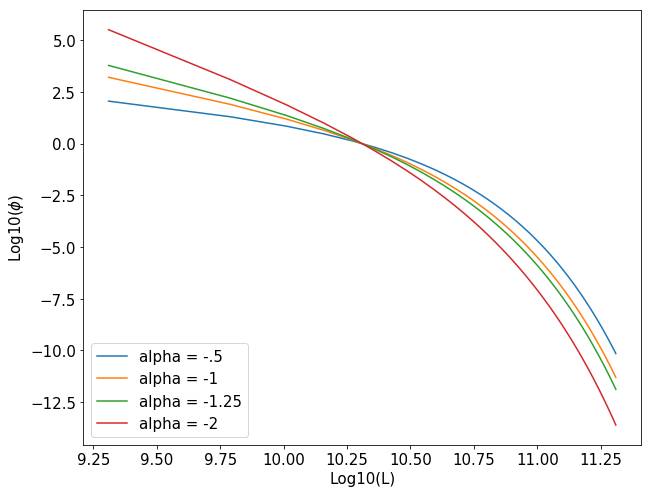
\includegraphics[width=5in]{scheter.png}
\caption{Scheter functions for different values of $\alpha$}
\end{figure}

\subsection{LMC to Milky Way ratios}
From the Milky Way + LG lectures, the V band luminosity of the Milky Way is $1.5 \times 10^{10} L_{\odot}$ and V band luminosity of the LMC is $1.7 \times 10^{9} L_{\odot}$. For a given $\alpha$ the ratios of the Scheter function evaluated at the LMC and MW luminosity will be

$$ \Big( \frac{L_{LMC}}{L_{MW}}\Big)^{\alpha} \exp(\frac{L_{MW} - L_{LMC}}{L_{*}}) $$

We will assume $L_{*B} \approx L_{*V}$. For $\alpha =  -.5, -1, -1.25,  -2$ I get 3.3, 16.93, 29.18, and 149.39, respectively.

\subsection{Convergence}
We can use the Scheter function to get the Luminosity density by introducing a factor of $L/L_* $ in the integrand

$$ n_* \int^{\infty}_0 (L/L_*)^{\alpha + 1} \exp(-L/L_*) \mathrm{d}\Big(\frac{L}{L_*}\Big) $$

If we make the substitution $z - 1 = \alpha +1$, this is the gamma function 

$$ n_* \int^{\infty}_0 (L/L_*)^{z -1} \exp(-L/L_*) \mathrm{d}\Big(\frac{L}{L_*}\Big) = n_* \Gamma(z)$$

The gamma function does not converge for negative values of z. From our definition, negative values of z correspond to $\alpha \leq -2$. All together, this means the Luminosity density is not convergent for $\alpha$ less than -2.

\subsection{SDSS data}
Please see figure 2 for the histogram.

The bins at lower redshift have larger populations of fainter galaxies. Observationally, this makes sense, since fainter galaxies placed further away are more difficult to detect. Furthermore, in the scaled version of the histogram one can see the higher redshift bins are more skewed towards the bright end. If there are relatively more galaxies brighter than -21 in the higher redshift bins, it may be an indication galaxies were brighter in the past. Lastly, the high redshift bins include more galaxies. This is expected, since the slices of the 'redshift cone' include more and more volume for higher redshift, given a fixed redshift slice. 

\begin{figure}
\centering
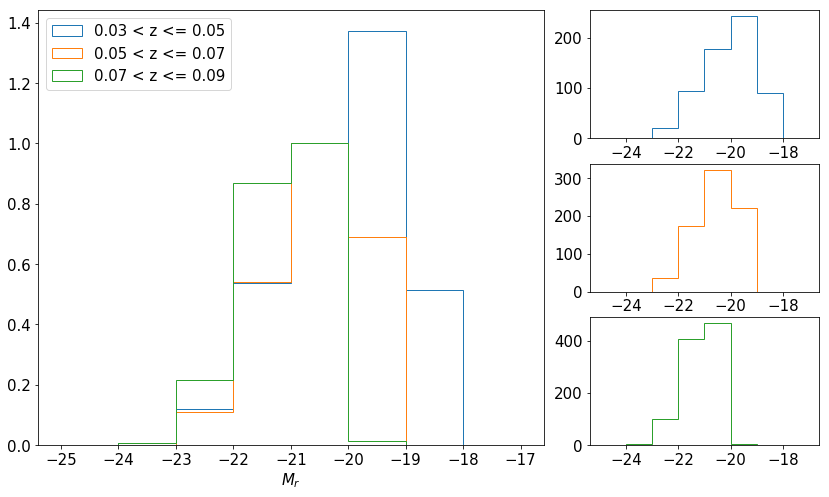
\includegraphics[width=5in]{redshifts.png}
\caption{Histograms of absolute r magnitude for three different redshift bins. In the largest panel on the left, all the histograms have been normalized such that $M_{r} = -21$ has a height of 1. The right column shows the individual bins plotted individually, with no normalization, for clarity.}
\end{figure}

\section{Stromgren Sphere}
\subsection{$r_*$ for a mid-O star}
The radius of the Stromgren sphere is given by

$$r_* = (3N_* / 4\pi \alpha n_e^2)^{1/3}$$

Plugging in the numbers gives us a value of $2.29 \times 10^{18} \mathrm{cm}$ 

The gas mass is given by multiplying the mass of hydrogen by the number density by the volume of the Stromgren sphere

$$M_{gas} = \frac{4\pi}{3} r_*^3 n_* m_{H}  = \frac{4\pi}{3} (2.29 \times 10^{5})^3 \times 10^3 \times 1.67 \times10^{-24} = 8 \times 10^{25} \mathrm{g}$$

\subsection{Scaling relationships to $r_*$}

$r_* \propto n_e^{-2/3}$, so by increasing the density by a factor of 10 the Stromgren radius goes down by $10^{-2/3} \approx .215$. The mass is proportional to $r_*^3$ and $n_e^{-2}$ by extension. Increasing the particle density by a factor of 10 decreases the mass by a factor of 100

\subsection{$r_*$ for a B1 star}
If we fix the temperature and number density but adjust $N_*' = N_* \times 3 \times 10^{-2}$, our new $r_*$ will scale as $(3 \times 10^{-2})^{1/3} =.31$. So our new radius is $7.1 \times 10^{17}$ cm.

\subsection{He+ and H+}
The energy required to singly ionize Helium is almost twice as much as the ionization energy of Hydrogen. And, while any photon emitted that can ionize Helium can also ionize Hydrogen, the opposite is not true. Helium atoms need to compete with Hydrogen for ionizing photons in this sense, while Hydrogen is able to become ionized by an additional pool of lower energy photons. As a result, more Hydrogen atoms will be ionized than Helium atoms, and the Stromgren sphere for HII will be larger than for HeII. 

\section{ISM}
\subsection{Pressure equilibrium}
We can calculate the pressures of these systems by using the ideal gas law, $PV = NKT$ or $P = nKT$ where $n$ is particle number density. For the ionized gas we get $6\times10^{3}  \times 5\times10^{5} \times 1.38064852 \times 10^{-23} = 4.14 \times 10^{-14} \mathrm{Pa}$.
For the cold molecular gas we have  $50 \times 2\times 10^{7} \times 1.38064852 \times 10^{-23} = 1.38 \times 10^{-14} \mathrm{Pa}$.
For the warm gas we have $ 10^4 \times 10^5   \times 1.38064852 \times 10^{-23} = 1.38 \times 10^{-14}\mathrm{Pa}$
Since the warm and cold gas have the same pressure, they are in pressure equilibrium.

\subsection{What happens next?}
I thought about this for a while, and admittedly my explanation is a bit hand-wavy. Ultimately, I think the entire system will move to an equilibrium state where the pressures are equal. Assuming we have a way to keep the gases from mixing, and they are not free to keep expanding into space, at the interface where the hot ionized gas meets the warm neutral gas, there is a pressure imbalance, which means there is a net force. The pressures at the interfaces will then adjust themselves until they are equal, so there is no imbalanced force. This will then have to happen at the interface between the warm and cold gas, until the entire system is in equilibrium. This has to happen by tweaking the temperatures and particle densities in the different systems. We can explain this by zooming in on the interfaces, and imagining particle collisions between the ions and warm gas helping to raise the warm gas temperature, and thus pressure. The same can be said of the interface between the cold molecular gas and warm neutral gas. 

\subsection{What else is contributing to this system?}
The source of ionizing photons that gives rise to the ionized gas plays a part in this as well. Photons carry momentum and can exert pressure. Additionally, the rate at which ionizing photons are produced effects the temperature and particle density of ions, and its pressure by extension. 

\section{Galaxy Spectra}
\subsection{Match spectra to images}
The middle galaxy is an elliptical. These are supposed to be 'red and dead', meaning their star formation ceased long ago, and their stellar populations are dominated by red K stars. For this reason, the bottom most spectra must correspond to it, since it looks like a K star template spectra. What few emission features there are, are not very high compared to the continuum, and there are many absorption features.

The remaining galaxies are a spiral and a merging galaxy. We know mergers lead to intense star formation, so the spectrum of the remaining two which indicates greater star formation must match galaxy 3. For this reason, I think spectrum a goes with galaxy 3. The Balmer series lines in spectra a have greater intensity relative to the continuum than for spectra b. This indicates the HII regions in this galaxy are contributing more relative flux, which in turn suggests high star formation rates. This leaves galaxy 1 being paired with spectrum b. This spectrum has HII regions, which are not as intense as the starburst galaxy. Additionally, there are some of the absorption features from the elliptical spectrum are present here, indicating a population of evolved K stars. This fits the bill, since we know spirals will have some old evolved stars, but are gas rich enough to support some star formation. 

\subsection{How would the images look if they were in color?}
The elliptical luminosity is dominated by K stars, the starburst galaxy by O and B stars, and the spiral is somewhere in between. The elliptical should look red, while the spiral will be bluer, and the star burst galaxy very blue.
\end{document}